\documentclass[a4paper,12pt]{article}
\usepackage[utf8]{inputenc}
\usepackage[brazil]{babel}
\usepackage[hidelinks]{hyperref}
\usepackage{indentfirst}
\usepackage{listings}
\usepackage{graphicx}
\usepackage{float}
\usepackage{color}
\usepackage{xcolor}
\usepackage[final]{pdfpages} %for including pdf file pages in latex
\hypersetup{
	colorlinks,
	linkcolor={red!100!black},
	citecolor={blue!50!black},
	urlcolor={blue!80!black}
}

\newcommand{\thecompany}{\huge Documentação em português}
\newcommand{\thelogo}{\begin{figure}[H] \centering \includegraphics[height=3cm]{BRASAOUFV.jpg} \end{figure}}
\newcommand{\thedate}{\today}
\newcommand{\thetitle}{\textbf{\LARGE  Projeto BusinessSysMan} \\ \large{Gerenciador de Empresas Livre}}
\newcommand{\theauthor}{Veloso G., Victor e Vieira G.,Fadoa}
\definecolor{listinggray}{gray}{0.9}
\definecolor{lbcolor}{rgb}{0.9,0.9,0.9}
\lstset{
	tabsize=4,
	language=[GNU]C++,
	basicstyle=\scriptsize,
	upquote=true,
	aboveskip={1.5\baselineskip},
	columns=fixed,
	showstringspaces=false,
	extendedchars=false,
	breaklines=true,
	prebreak=\raisebox{0ex}[0ex][0ex]{\ensuremath{\hookleftarrow}},
	frame=single,
	numbers=left,
	showtabs=false,
	showspaces=false,
	showstringspaces=false,
	keywordstyle=\color[rgb]{0, 0, 1},
	commentstyle=\color[rgb]{0.026,0.112,0.095},
	stringstyle=\color[rgb]{0.627, 0.126, 0.941},
	numberstyle=\color[rgb]{0.205,0.142,0.73}
}
\lstset{
	backgroundcolor=\color{lbcolor},
	tabsize=4,
	language=C++,
	captionpos=b,
	tabsize=3,
	frame=lines,
	numbers=left,
	numberstyle=\tiny,
	numbersep=5pt,
	breaklines=true,
	showstringspaces=false,
	basicstyle=\footnotesize,
	keywordstyle=\color[rgb]{0, 0, 1},
	commentstyle=\color{Darkgreen},
	stringstyle=\color{red}
	}
\begin{document}
	
	\begin{titlepage}
		\begin{center}
			\thecompany
			
			%\thelogo
			
			\vspace{10pt}
			
			
			\vspace{60pt}
			
			\thetitle
			
			\vspace{160pt}
			
		\end{center}
		
		\begin{flushleft}
			\begin{tabbing}
				Organizadores\qquad\qquad\= \theauthor \\
				Patrocinadores\> Recondicionadora Nacional; Retífica Dobber\\
				
			\end{tabbing}
			
		\end{flushleft}
		
		\begin{center}
			\vspace{\fill}
			Brasil, MG - Belo Horizonte, 2017%\thedate
		\end{center}
	\end{titlepage}
	\tableofcontents
	\thispagestyle{empty}
	\clearpage
	\setcounter{page}{1}
	\begin{abstract}
	Este projeto tem o intuito de facilitar a administração financeira e de funcionários de pequenas, médias e grande Empresas sem nenhum custo e com total liberdade de alteração e distribuição. Inicialmente baseada na framework multiplataformas e multiarquiteturas Qt, buscamos o máximo de acessibilidade e compatibilidade com a menor curva de aprendizado e adaptação para que a consulta aos dados seja um possibilidade a todos. Todos arquivos estão disponibilizados em um \href{https://github.com/primary157/TP1AEDS1.git}{repositório do GitHub} com cada etapa do processo de criação. 
	\end{abstract}
	\section{Metodologia}
	
		\subsection{Organização e Planejamento do Projeto}
			O trabalho foi dividido em 3 fases: 
			\begin{enumerate}
				\item a fase de planejamento;
				\item a fase de produção e elaboração dos casos de teste;
				\item a fase de conclusão.
			\end{enumerate}
			\subsubsection{Fase de Planejamento}
			Na fase de planejamento elaboramos diagramas que representariam a estrutura do programa, a lógica a ser implementada e "rascunhos" de como seria a aparência das "telas" do programa, além de estudarmos as ferramentas que melhor auxiliariam na solução do problema proposto.
			\subsubsection{Fase de produção e elaboração dos casos de teste}
			Esta fase é composta por 3 etapas:
			\begin{enumerate}
				\item Criação de testes unitários para garantir estabilidade e correspondência ao planejamento feito na fase anterior;
				\item desenvolvimento do código garantindo o sucesso dos testes criados;
				\item aperfeiçoamento do código buscando maior legibilidade e menor complexidade de processamento. 
			\end{enumerate}
			\subsubsection{Fase de conclusão e distribuição}
			Nesta fase iremos rodar o programa em várias arquiteturas estudando seu comportamento e reparando onde forem encontrados problemas, logo em seguida iremos empacotar para as maiores distribuições linux.
		\subsection{Ferramentas utilizadas}
		Durante a execução do projeto foi necessária a utilização de diversas ferramentas (listadas na tabela 1).
		\begin{table}[h]
			\label{table:tools}
			\resizebox{\textwidth}{!}{%
				\begin{tabular}{|lll|}
					\hline
					Nome                & Function                  & Função                               \\ \hline
					Tex-Studio          & Writing Documentation     & Escrever Documentação                \\ \hline
					GoogleTest             & Unit-testing              & Teste unitário                       \\ \hline
					cmake               & Cross-platform compiling  & Compilação multiplataforma           \\ \hline
					draw.io             & UML Designer              & Desenhar UML                         \\ \hline
					tablesgenerator.com & Generate LaTeX tables     & Gerador de tabelas LaTeX             \\ \hline
					Github              & Version-control           & Controle de Versão                   \\ \hline
					IRC           & Chatting and code sharing & Contato e compartilhamento de código \\ \hline
				\end{tabular}%
			}
			\caption{Lista de Software e Ferramentas}
		\end{table}
	\section{Diagramas, Licença e Códigos fontes utilizados}
		\subsection{Diagramas}
		\begin{figure}[H]
			\centering \includegraphics[width=\textwidth]{./ClassDiagramEnglish.pdf} 
		\end{figure}
		\begin{figure}[H]
			\centering \includegraphics[width=\textwidth]{./DiagramaDeClassesPortugues.pdf}
		\end{figure}
		\begin{figure}[H]
			\centering 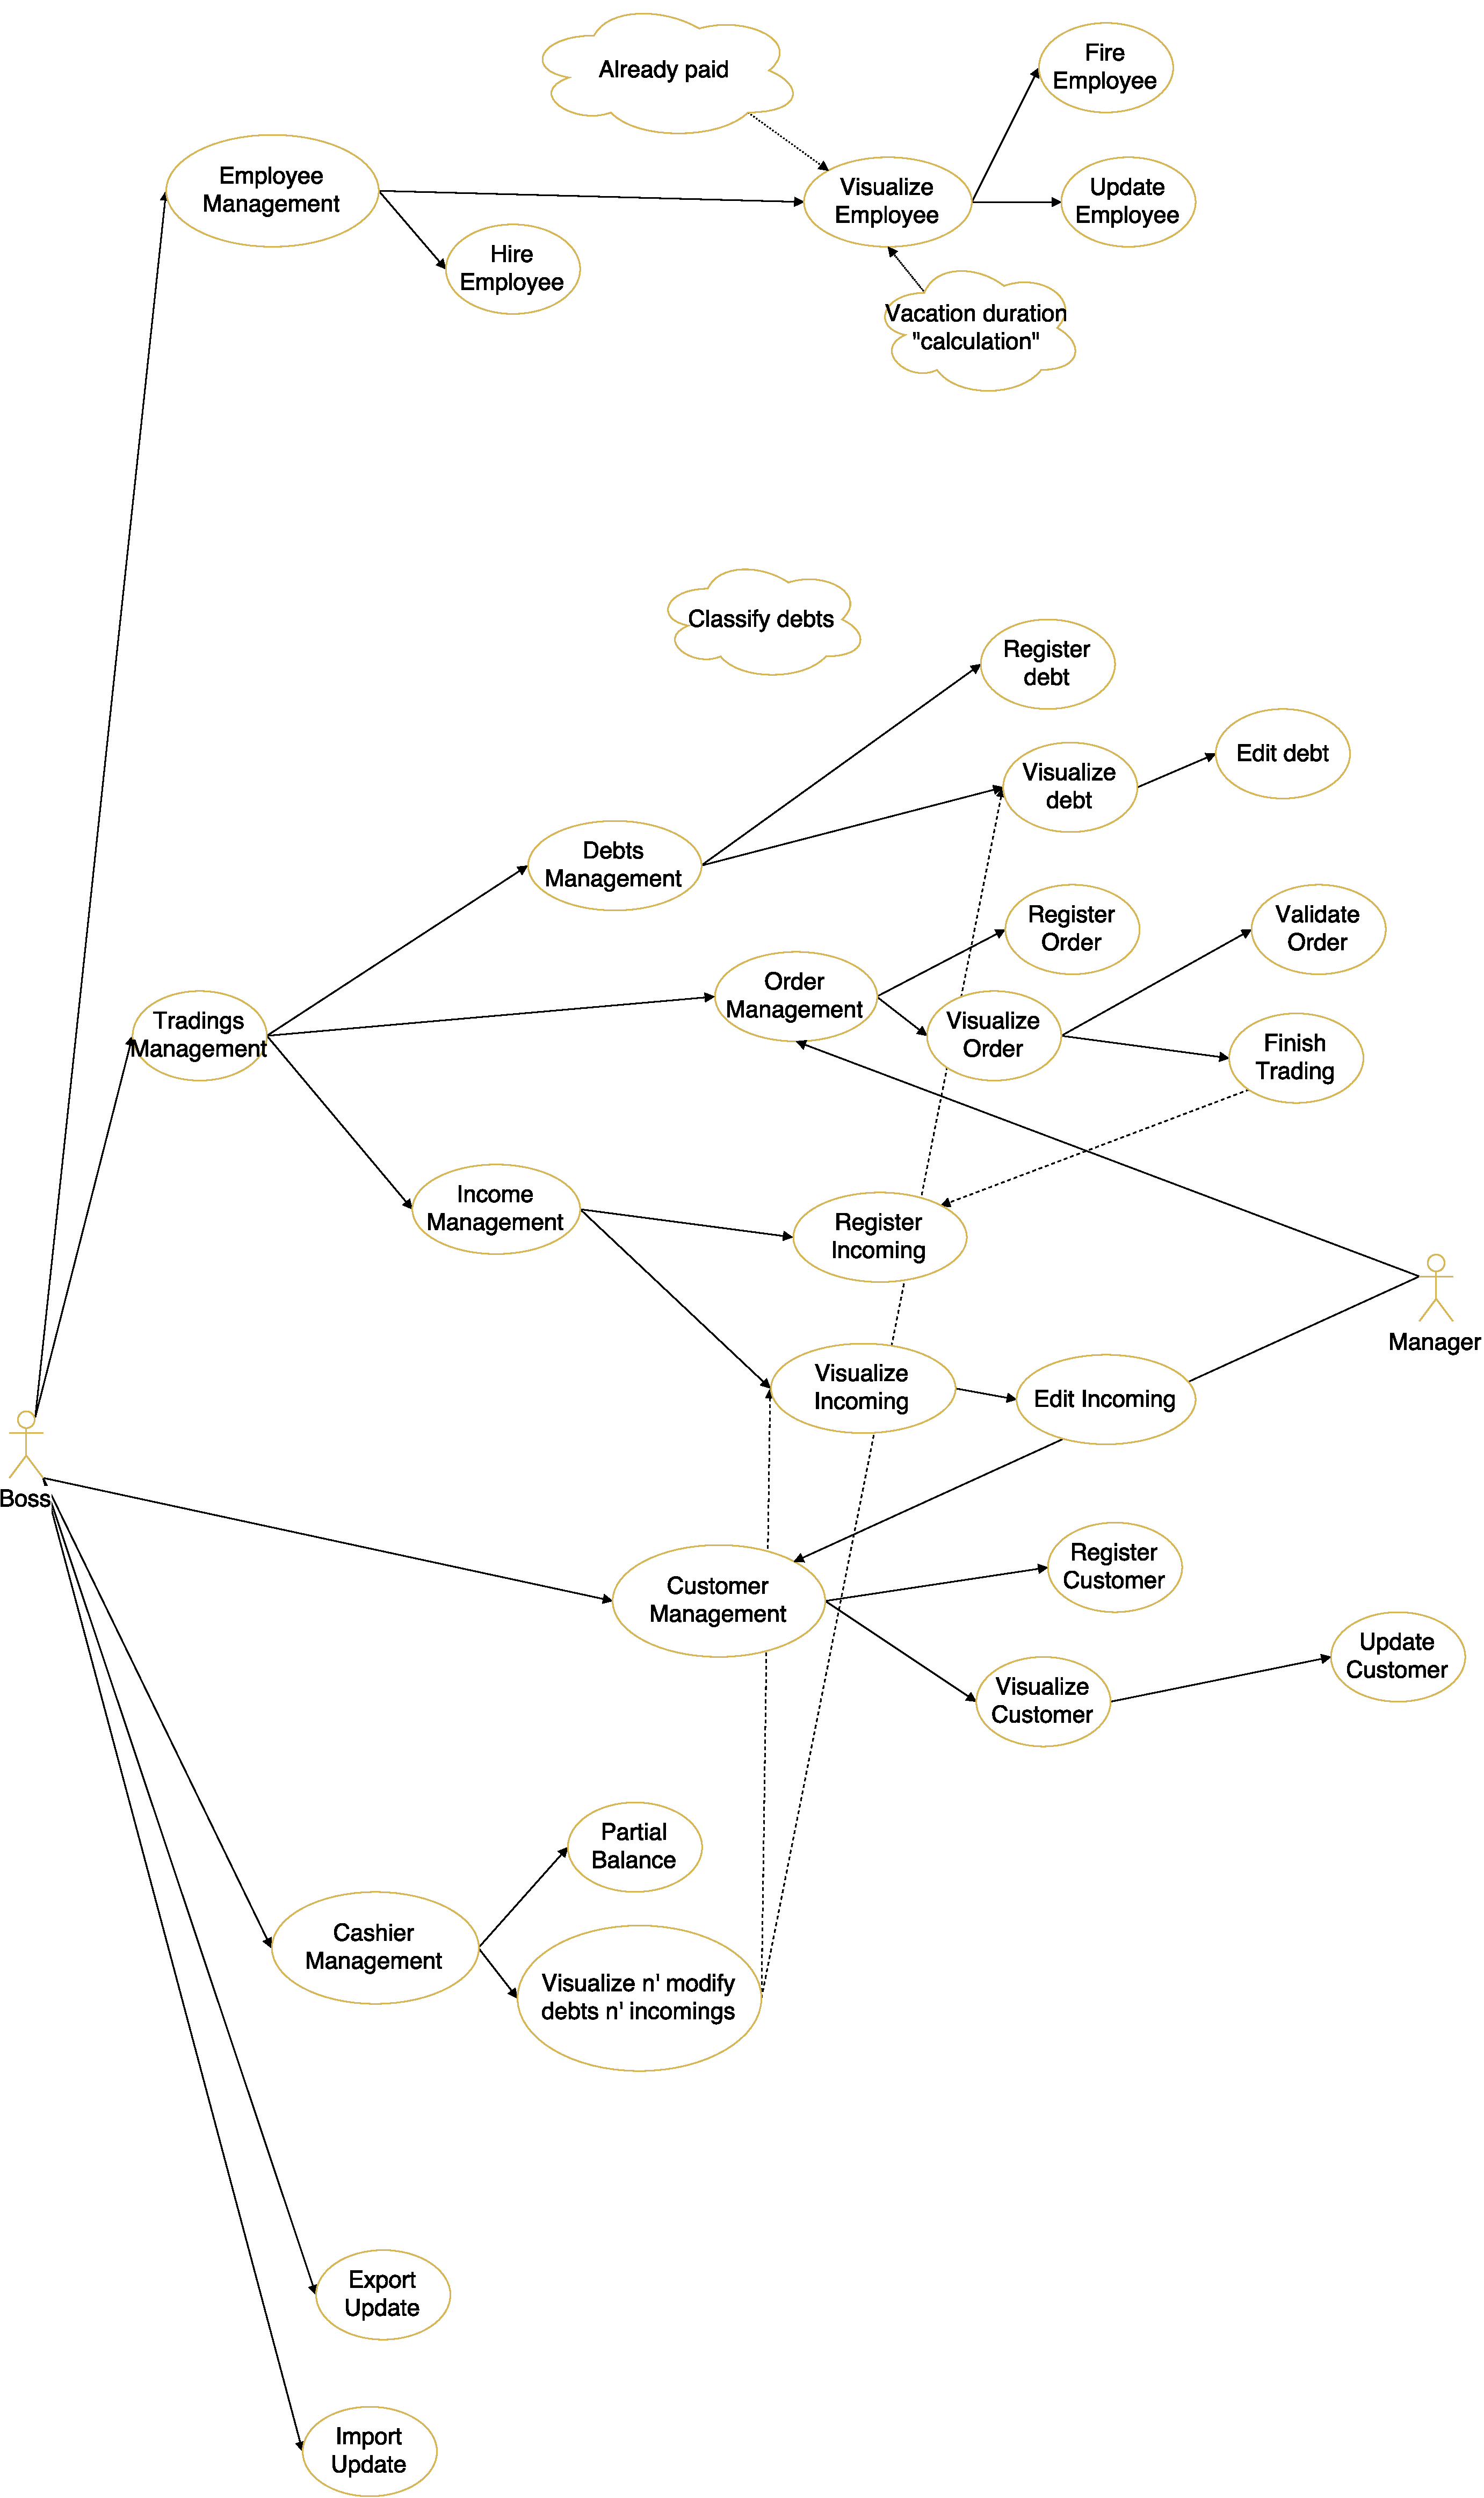
\includegraphics[width=\textwidth]{./UseCasesDiagramEnglish.pdf}
		\end{figure}
		\begin{figure}[H]
			\centering 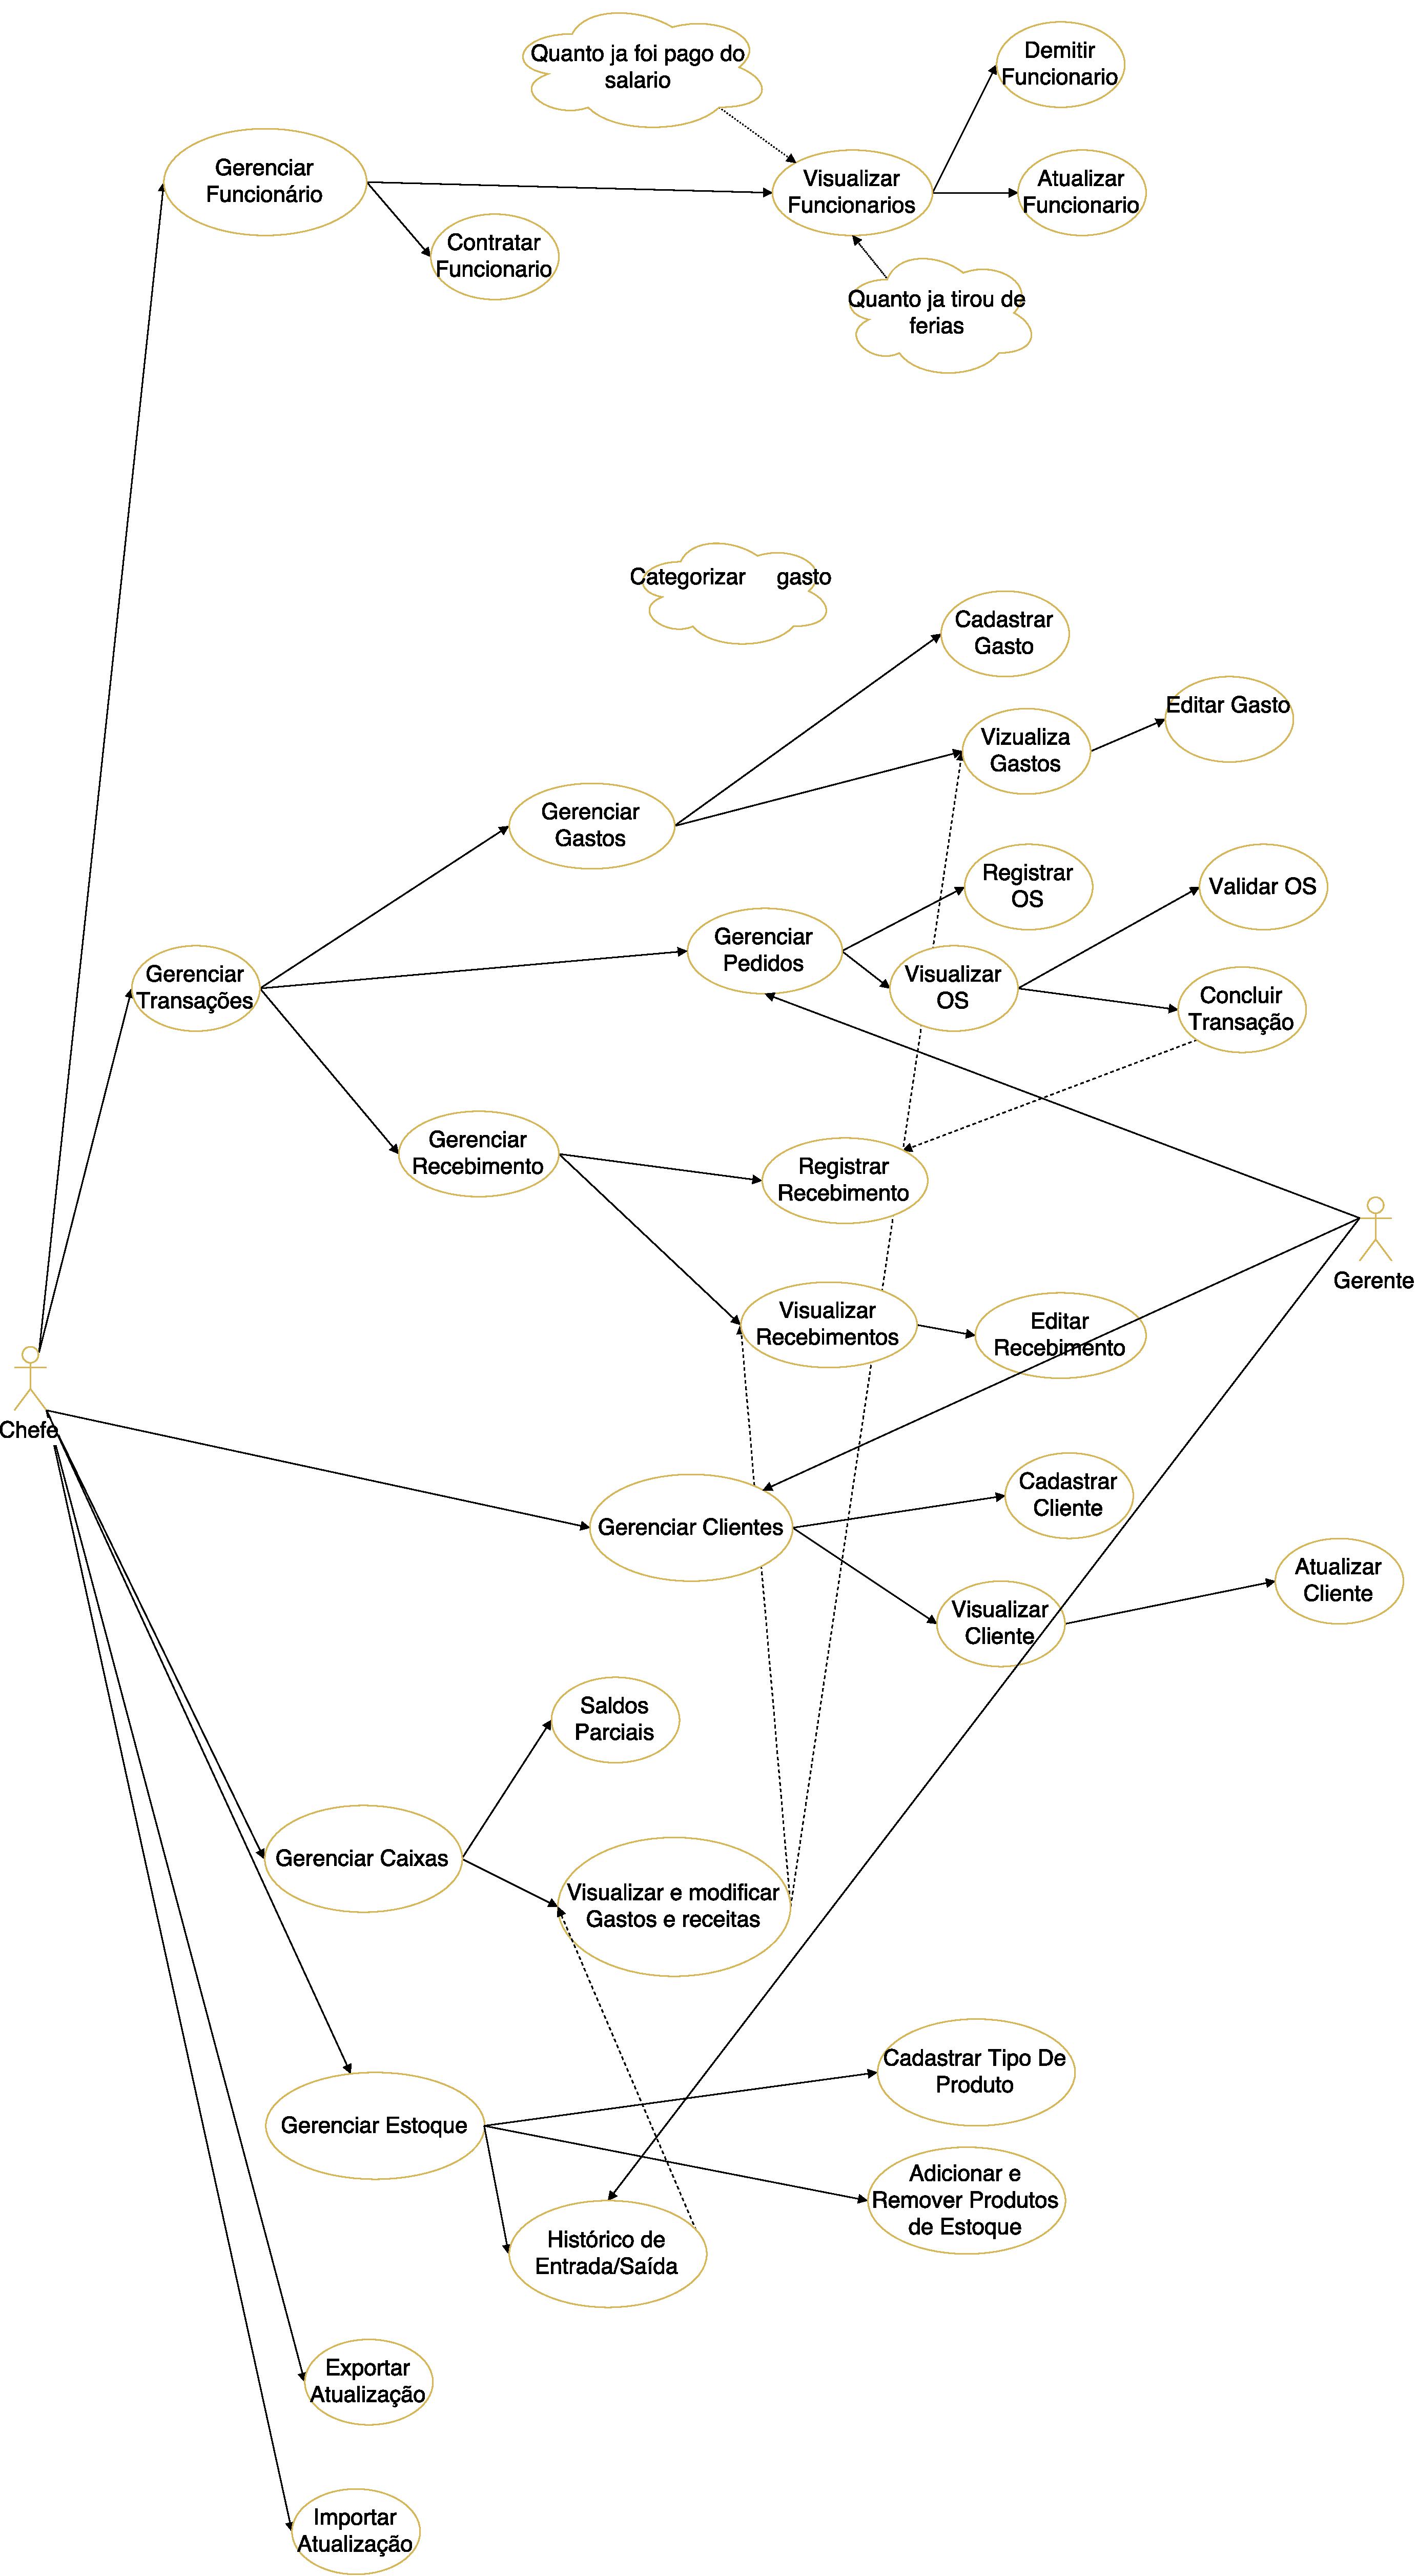
\includegraphics[width=\textwidth]{./DiagramaCasoDeUsoOficinaOld.pdf} 
		\end{figure}
		\begin{figure}[H]
			\centering 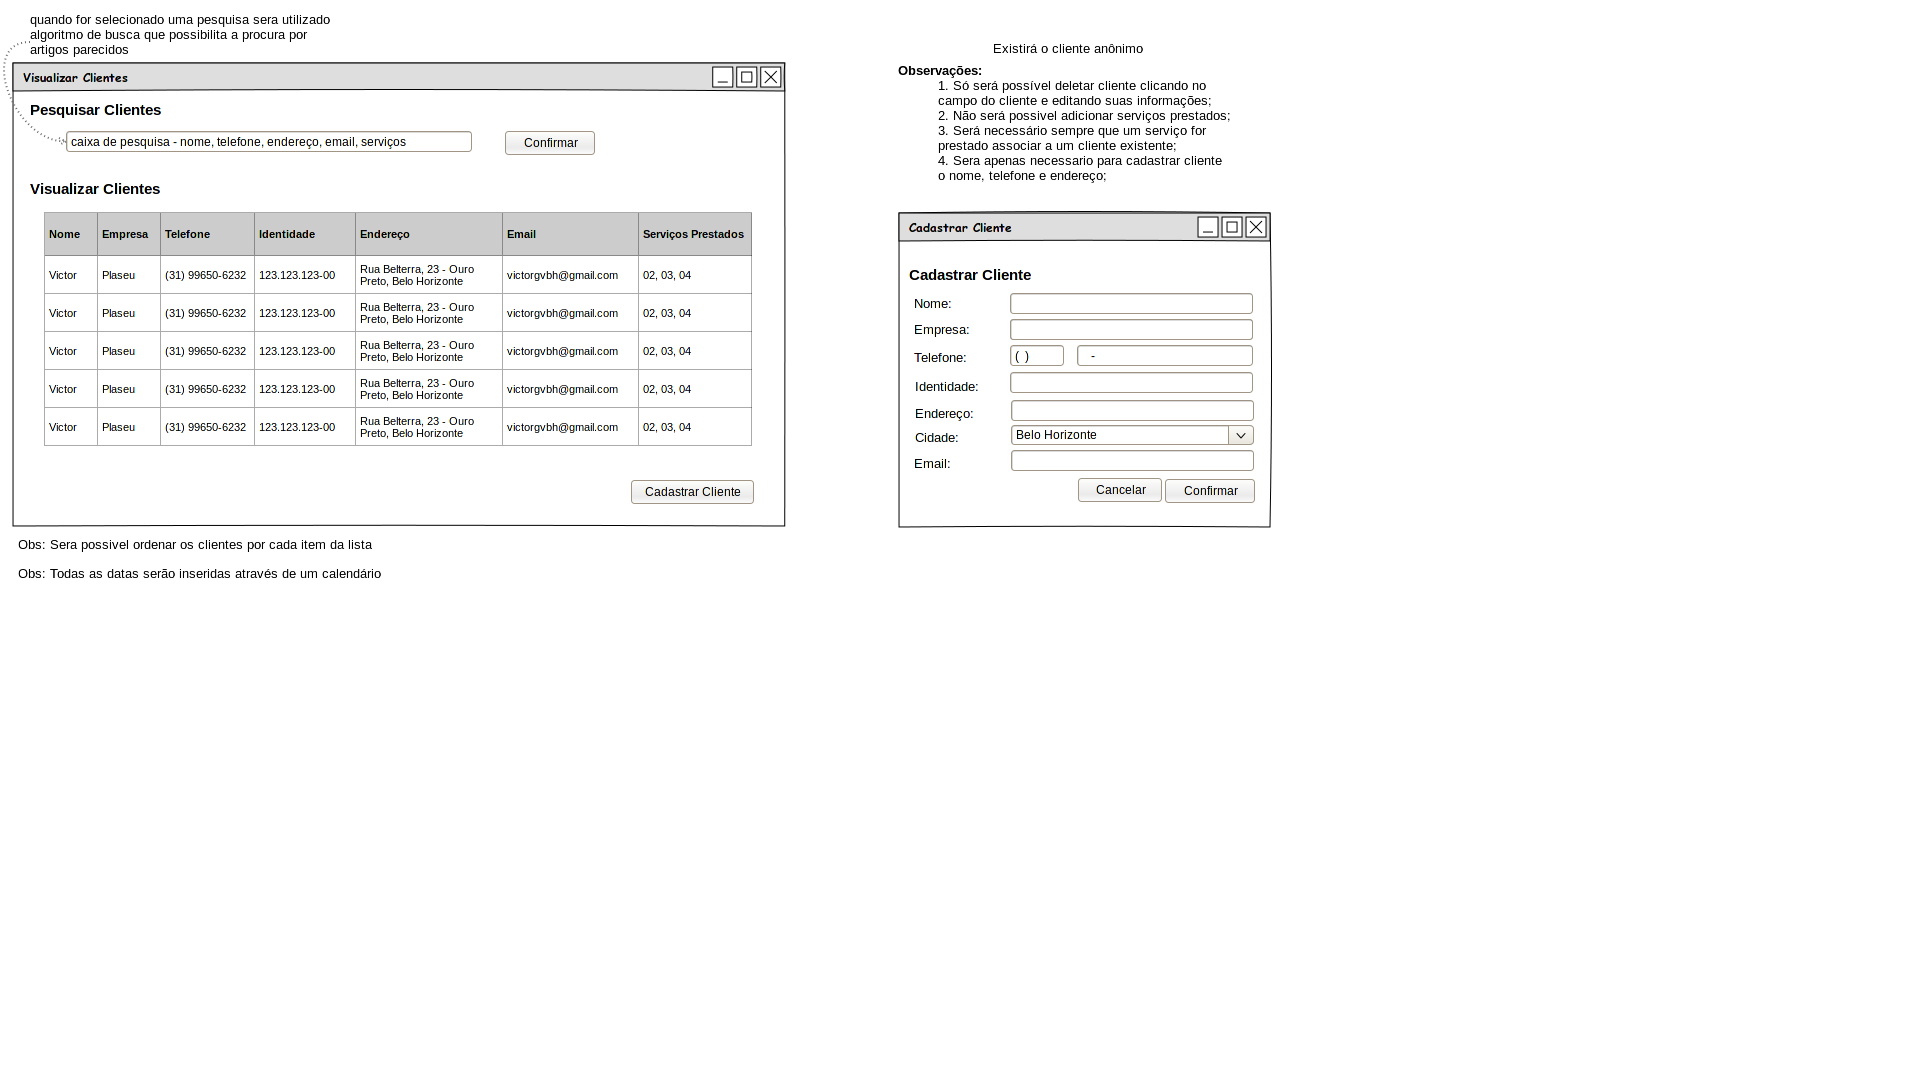
\includegraphics[width=\textwidth]{./Gerenciar Cliente.png}
		\end{figure}
		\begin{figure}[H]
			\centering 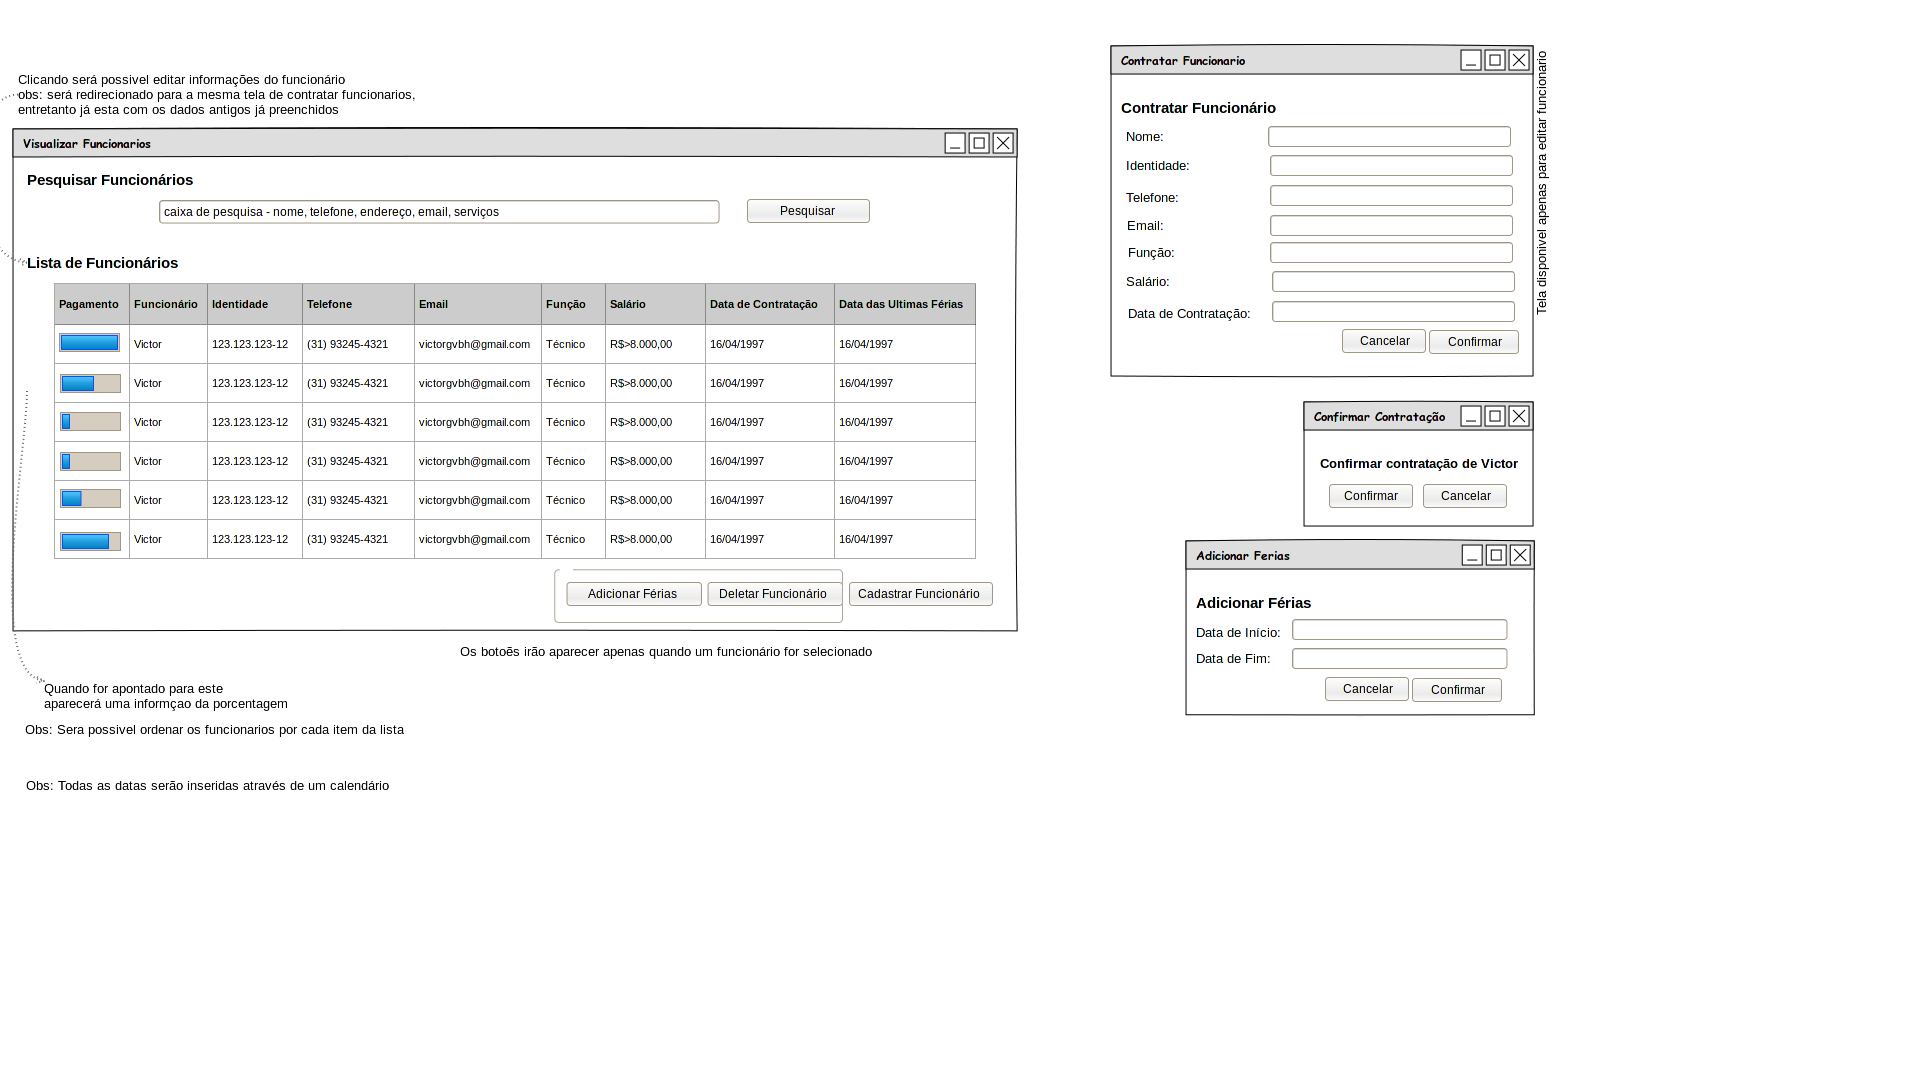
\includegraphics[width=\textwidth]{./Gerenciar Funcionario.png} 
		\end{figure}
		\begin{figure}[H]
			\centering 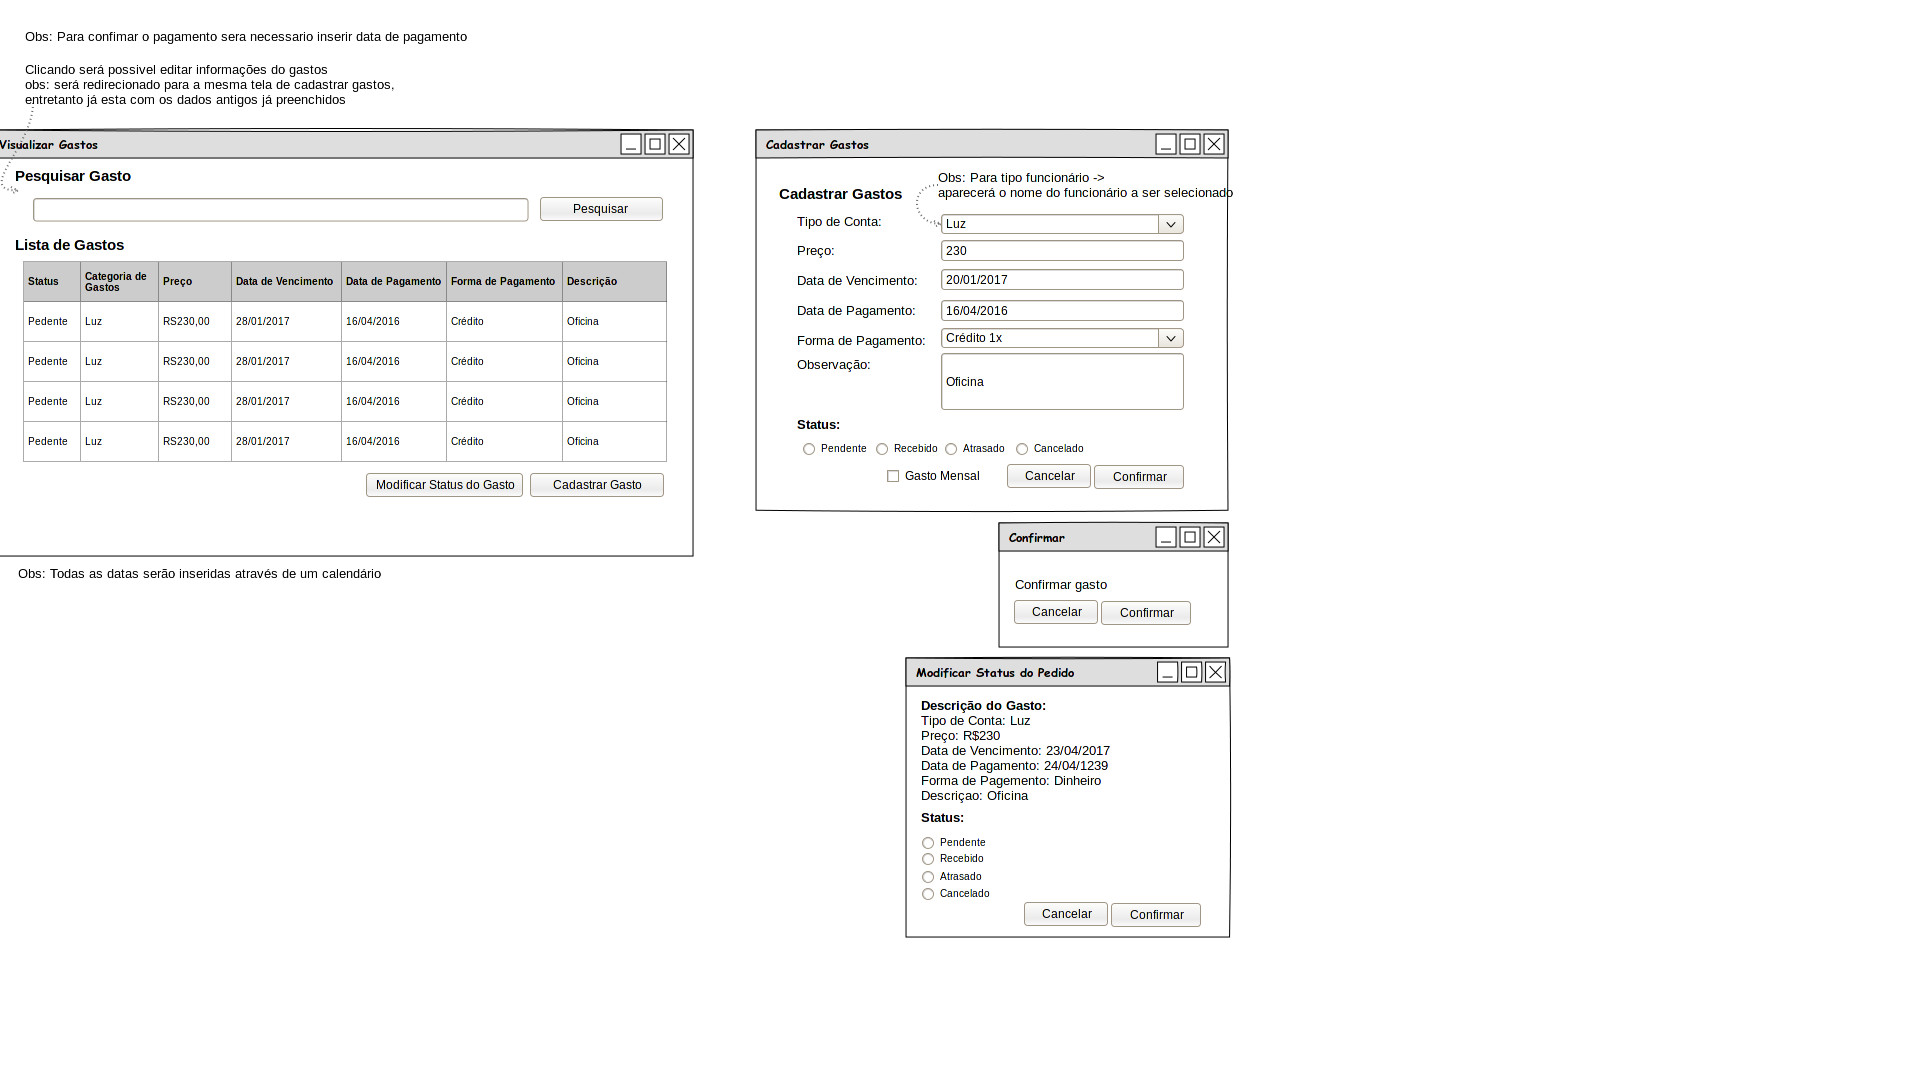
\includegraphics[width=\textwidth]{./Gerenciar Gastos.png} 
		\end{figure}
		\begin{figure}[H]
			\centering 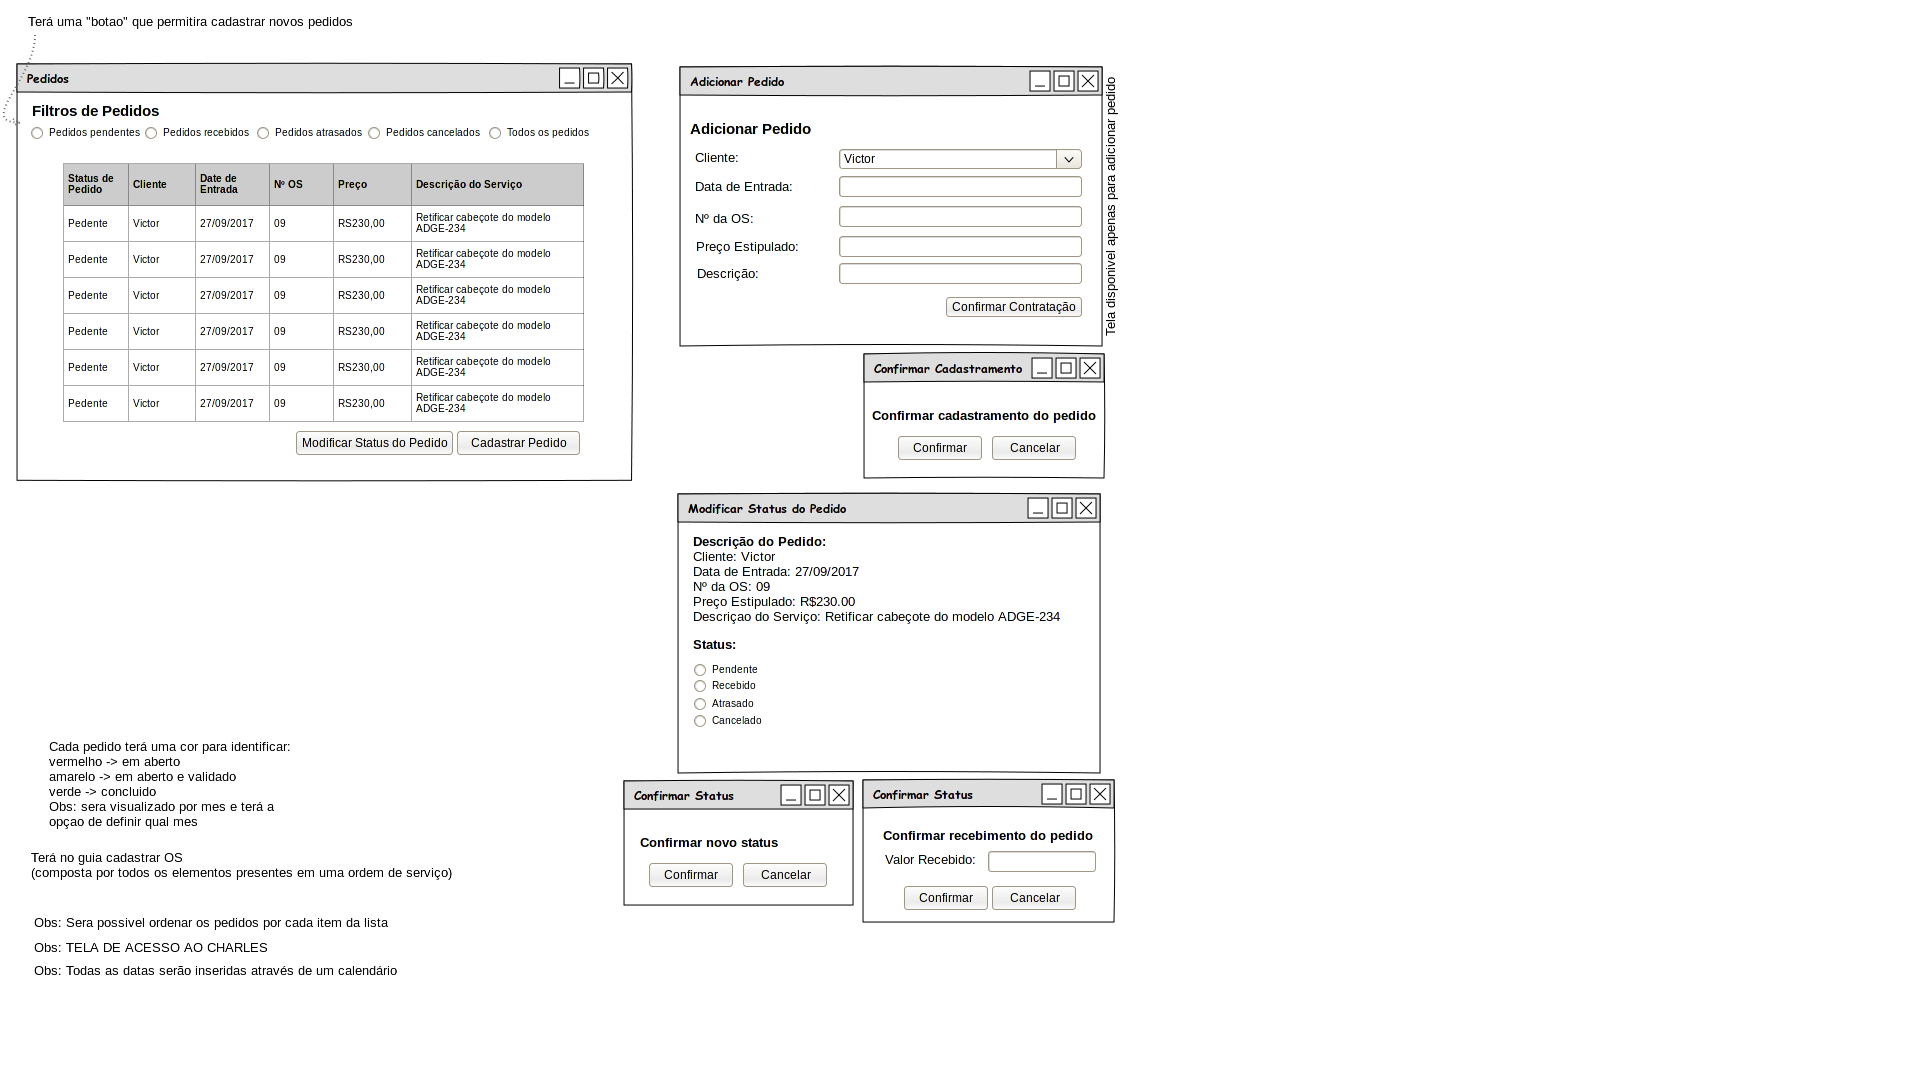
\includegraphics[width=\textwidth]{./Gerenciar Pedidos.png}
		\end{figure}
		\subsection{Licença} 
		
\includepdf[pages=-]{./lgpl-3-0.pdf}
		\subsection{Códigos Fontes incorporados ao programa}
		
		Por Enquanto Nenhum...
		
	\section{Tutoriais e FAQ}
		\subsection{Como contribuir para o projeto?}
		A contribuição pode ser feita de diferentes formas:
		\begin{enumerate}
			\item Utilizando e reportando bugs ou dando ótimas idéias de \textit{features} que podem ser incorporadas ao projeto;
			\item Contribuindo informalmente: caso você já possui algum código a ser incorporado ao projeto não perca seu tempo com formalidades, envie um pull request e um de nossos contribuidores irá estudá-lo e aceitá-lo caso realmente nos atenda;
			\item Contribuindo formalmente: você também pode se tornar um de nossos contribuidores formais! Basta entrar em contato com um dos organizadores (Primary157, MessiahG), para mais informações de como contactar-nos vá até a seção "Como contactar os organizadores?"
		\end{enumerate}
		\subsection{Como contactar os organizadores?}
		A seguir uma lista de contatos que criamos exclusivamente para o público deste projeto:
		 \begin{enumerate}
		 	\item Facebook:
		 	\item Email:
		 	\item IRC:
		 	\item Twitter:
		 \end{enumerate}
		Se não foi atendido como esperava ou não recebeu atendimento algum, também disponibilizamos aqui uma lista de meios para entrar em contato com cada um de nós individualmente:
			\subsubsection{MessiahG}
			\begin{enumerate}
				\item Email: fadoa.glauss@gmail.com
				\item IRC:
				\item Whatsapp:
				\item Github:
			\end{enumerate}
			\subsubsection{Primary157}
			\begin{enumerate}
				\item Email: victorgvbh@gmail.com
				\item IRC:
				\item Whatsapp:
				\item Github:
				\item Twitter:
			\end{enumerate}
		\subsection{Qual expectativa da data de conclusão?}
			Está cedo demais para pensarmos numa conclusão, além do mais que mesmo quando atingirmos as metas elaboradas no início do projeto ainda estaremos ativos elaborando cada vez mais metas para atendermos cada vez mais ao público empresarial.
		\subsection{Como instalar esse software?}
			Infelizmente não possuímos uma versão utilizável do programa. Mas não desanime! Manteremos você atualizado com oque acontece no projeto por meio das redes sociais Twitter e Facebook!
		\subsection{Como utilizar esse software?}
			Assim que ele obter uma versão utilizável é aqui que se encontrará o manual para o usuário final!
		\subsection{Como adotar esse software em minha empresa? Existe algum tipo de suporte?}
			Infelizmente não podemos te dizer se chegaremos a oferecer suporte algum dia. Mas se esse dia chegar lhe informaremos por meio das redes sociais!
		\subsection{Já baixei e utilizei, mas encontrei problemas ou coisas que poderiam ser adicionadas. Como entro em contato?}
			Vide subseção Como contribuir para o projeto? a algumas linhas acima!
		\subsection{Qual a vantagem de utilizar esse software?}
			Você estará contribuindo para uma comunidade de desenvolvedores que buscam tornar mais acessível a implementação de tecnologia na gestão de empresas. Além de estar economizando, por esse ser um software completamente gratuito.
		\subsection{Por que C++, Qt e SQLite?}
			Nossa equipe busca os melhores resultados possíveis, mesmo que o custo em tempo e desenvolvimento sejam maiores. Por esse motivo escolhemos a linguagem C++ que é uma linguagem de alto nível compilável que da muito poder ao desenvolvedor. 
			
			Como buscamos a acessibilidade não há nada mais interessante do que ser capaz de rodar o programa em qualquer arquitetura ou sistema operacional. Para isso optamos pela framework Qt que oferece as características citadas com a garantia de ter a mesma aparência e funcionalidades em todos os sistemas, essa framework possui sua versão com licença completamente livre e promete entregar uma interface responsiva e muito agradável aos olhos. 
	\section{Referência}
	%TODO Fazer a referencia
	\section{Agradecimentos}
		Obrigado a todos, que nos apoiaram no momento de criação e elaboração deste projeto, sem o apoio de vocês provavelmente esse projeto estaria agora se preparando para um descanso eterno em uma de nossas gavetas.
		
		Ah e para aqueles que entrarem depois no projeto não pense que esquecemos de vocês, então se seu nome não se encontra na lista abaixo a culpa é exclusivamente sua, então trate logo de fazer um pull request adicionando-o.
		
		Desenvolvido por: Amaury, ZecaTapado, FadoaGlauss, Primary157, Astopho, Ramon, Daniel, Gabriel, Indiano, Lucas, Pedro, Zenon...
\end{document}
